\documentclass{article}

% if you need to pass options to natbib, use, e.g.:
% \PassOptionsToPackage{numbers, compress}{natbib}
% before loading nips_2017
%
% to avoid loading the natbib package, add option nonatbib:
% \usepackage[nonatbib]{nips_2017}

\usepackage[final, nonatbib]{nips_2017}

% to compile a camera-ready version, add the [final] option, e.g.:
% \usepackage[final]{nips_2017}

\usepackage[utf8]{inputenc} % allow utf-8 input
\usepackage[T1]{fontenc}    % use 8-bit T1 fonts
\usepackage[hidelinks]{hyperref}       % hyperlinks
\usepackage{url}            % simple URL typesetting
\usepackage{booktabs}       % professional-quality tables
\usepackage{amsfonts}       % blackboard math symbols
\usepackage{nicefrac}       % compact symbols for 1/2, etc.
\usepackage{microtype}      % microtypography
\usepackage{algorithm}
\usepackage{algorithmic}
\usepackage{subcaption}
\usepackage[numbers]{natbib}
\usepackage{graphicx}

\title{DQN: Learning To Learn}

% The \author macro works with any number of authors. There are two
% commands used to separate the names and addresses of multiple
% authors: \And and \AND.
%
% Using \And between authors leaves it to LaTeX to determine where to
% break the lines. Using \AND forces a line break at that point. So,
% if LaTeX puts 3 of 4 authors names on the first line, and the last
% on the second line, try using \AND instead of \And before the third
% author name.

\author{
  Dennis Verheijden\\
  s4455770
  \And
  Joost Besseling\\
  s4796799
  %% examples of more authors
  %% \And
  %% Coauthor \\
  %% Affiliation \\
  %% Address \\
  %% \texttt{email} \\
  %% \AND
  %% Coauthor \\
  %% Affiliation \\
  %% Address \\
  %% \texttt{email} \\
  %% \And
  %% Coauthor \\
  %% Affiliation \\
  %% Address \\
  %% \texttt{email} \\
  %% \And
  %% Coauthor \\
  %% Affiliation \\
  %% Address \\
  %% \texttt{email} \\
}

\begin{document}
 %\nipsfinalcopy is no longer used

\maketitle

\begin{abstract}
We show that it is possible to implement a deep Q-network in Chainer. We use different techniques to train the network efficiently. We manage to achieve super human performance in a number of games and confirm that the original DQN scores are a solid baseline for future studies.
\end{abstract}

\section{Introduction}
Reinforcement learning is becoming a field in machine learning that is getting a lot of attention lately, with AlphaGo Zero beating the previous Go Champion, which was also an AI \cite{silver2017mastering}. The latter defeated the World Champion in Go. So currently, the best Go player in the world is an AI.

One of the first algorithms that successfully played a big range of games was proposed by \citep{mnih2013playing}, called Deep Q-Learning Networks (DQN). Here the AI was given the raw pixel values as input to the model. In this model, Q-values were used as an measure for how good an action is in a specific state.

This was made possible by Atari Gym \cite{1606.01540}, a reinforcement learning environment to train and test various reinforcement learning algorithms on difficult, real-time, tasks. The gym has a large variety of different games that are commonly used as a benchmark tool for testing models. Our goal was to implement and train a novel  reinforcment learning neural network in Chainer \cite{chainer_learningsys2015}. We chose to implemented deep Q-learning as introduced by \cite{mnih2013playing}, with extentions from \cite{mnih2015human}.

The structure of this paper is as follows: We will first give a short introduction to the problem of reinforcement learning. We then proceed with giving an overview of the various techniques that are proposed to train a deep Q-network and techniques to speed up learning. We then present our results and finish with an overview of our study with resulting conclusions.

\section{Background}

\subsection{Atari}

The Atari gym environment works as follows: An agent is playing a game, choosing different actions based on the current state (observation). When the agent manages to score a point, the game will return a reward. If the agent dies, the game will return a different reward. It is easy to see how this leads to difficulties, since there might not be a direct relation between the last action and the last reward. Scoring a point may be the cause of an action that happened 100 frames ago.

An example may be drawn from the game of Pacman. The agent has to make sure it is not trapped by the little ghosts. If it is trapped, it will not immediately die. Death will after a longer amount of frames. To make the problem even more complex: the immediate positive reward after eating a pallet in a corridor, might lead to the agents demise.

On a lower level, the Atari environment works as follows: it uses a default routine for all the games available. First it has to be initialized, after that we can iterate through the screen by calling the \texttt{step} function on the environment with the action that the agent wants to perform. The environment will then return the resulting state, the reward, whether the game is finished or not and some information that is game specific. When the game is finished, i.e. \textit{done} is \textit{True}, we reset the environment to start another game, or we stop and are done with the training.

\subsection{Reinforcement Learning}

As stated before, the Atari environment provides a specific learning environment. The agent receives positive or negative rewards and has to change its actions based on these rewards. This methodology is called reinforcement learning. Reinforcement learning differs from both supervised and unsupervised learning in a number of ways. It differs from supervised learning because we don't have a training set of labeled data, we only gain the `labels' after performing the action. In the context of Atari games, there is also a temporal mismatch between receiving a reward and whether the previous action is specifically the cause for gaining this reward.

It differs from unsupervised learning too, the network does receive information about whether the performed action was good or bad. So we are not simply learning the general structure of an Atari game, as is common in unsupervised methods.

This poses a number of different challenges. For example, the distance between an action and the reward. Also, the agent will explore different states of the game, based on the actions that it takes. This has as a consequence that there is a balance between exploration and exploitation, if the agent always chooses the same action that has an immediate reward, the agent might get stuck in the game. But if it acts too randomly it might not learn to get past a difficult part of the game, in which it has to take a dangerous action first \cite{reinforcementLearningDraft}.

\subsection{Q-learning}

One way to deal with the mentioned difficulties is Q-learning. Q-learning was proposed by \citeauthor{watkins1992q} \cite{watkins1992q}. The assumption of Q-learning is that there is some function called $Q(s, a)$ that provides the gain of doing action $a$ when the agent is in state $s$. If we assume that we have this function available, we can utilize it by evaluating it at every state and choosing the action with the highest value. This will then result in perfect play. The problem is, of course, that we don't know this $Q$-function. 

One approach to approximate the $Q$ function is the so called tabular Q learning. The main idea is to use the Bellman equation: 

\[
	Q(s_t,a_t) = (1 - \alpha) Q(s_t, a_t) + \alpha(r_t + \gamma \max_{a_{t+1}} Q(s_{t+1},a_{t+1})),
\]

here $s_t$ is our current state, $a_t$ is the chosen action, $r_t$ and $s_{t+1}$ are respectively the reward and next state resulting from performing action $a$. In tabular Q-learning, $Q$ is approximated by a table of size $S \times A$, where $S$ is the size of the state-space and $A$ is the size of the action space. 

Unfortunately, the state-space is really big in our environments, since every slight change of a single pixel value in the Atari games is seen as a different state. This problem makes tabular Q-learning not feasible for our project.

To tackle this specific problem, \citeauthor{mnih2013playing} proposed a solution: replace the table with a neural network for approximation. The neural network can then be trained to estimate the $Q$ function for every state. However, instead of having a separate network for each action, we will have an output layer corresponding to every possible action that can be performed. This leads to the new updating rule:

\[
    Q(s_t,a_t) = r_t + \gamma \max_{a_{t+1}} Q(s_{t+1},a_{t+1}))
\]


There are numerous challenges when training a deep Q-network. In this paper we will discuss a few of the problems that have to be considered and methods to combat these problems.

\subsection{Network Architecture}
%model beschrijven in termen van \emph{states rewards and actions} + Q-learning (is pure value iteration aka rewards propagaten van de terminal state naar de eerste zet in episodes)

The network architecture that we will be using has a number of different layers. Since we are dealing with raw pixel data, we have chosen to use three convolutional layers. Convolutional layers are especially good at handling visual input, because they take advantage of the the spatial features that are hidden in the pixel data. After these layers we have two fully connected layers. The size out the final fully connected layer corresponds to the number possible actions the agent can perform. After every hidden layer we perform a rectified linear activation function.



\section{Related Work}
%Not sure... Misschien wat vertellen over de guru paper \cite{mnih2013playing} + mogelijke verbeteringen in NATURE \cite{mnih2015human}

Reinforcement learning is a very active field, so there is a lot of related work. In \citeyear{mnih2013playing} \citeauthor{mnih2013playing} introduced a novel way to tackle the problem of reinforcement learning which they called Deep Q-learning. This method is highly effective, achieving super human play in a number of games \cite{mnih2013playing}. In \citeyear{mnih2015human}, \citeauthor{mnih2013playing} proposed a new iteration of their DQN algorithm with several new tricks to achieve higher highscores and make the learning process more stable \cite{mnih2015human}.

More recently, Google's Deepmind achieved another major success when they managed to beat the worlds best Go players, using a version of reinforcement learning and subsequently beating their own world champion with a new iteration of their AI \cite{silver2017mastering}.

Another problem of Neural Networks is the so called Catastrophic Forgetting which means that if we take a network, and train it on \textit{problem 1}, for example one of the games in Atari. And then train it on a different game, \textit{problem 2}, the network will `forget' how to play problem 1 \cite{rusu2016progressive}.

Anonther problem is that of knowlegde transfer. Some games are fairly similar, so learning one game might help you play another game. But can a neural network transfer the knowledge from one game to the next? There are a number of ways to tackle these problems. For example the work that \citeauthor{rusu2016progressive} did on Progressive Neural Networks \cite{rusu2016progressive}. In this paper they introduce a network architecture that adds a new network for every problem that it encounters, but incorporates all computations of the previous networks via lateral connections to previous hidden layers of previously learned tasks. The idea is that these computations speed up the learning of the next network, because some of the knowledge transfers from one game to the next.


\section{Methods}
Because deep q-learning is computationally expensive, we had to use a lot of optimizations and tricks to speed up the learning process. There is also a lot of instability in learning optimal Q-values, so we use some methods to reduce the combat this instability. In this section we will describe the techniques that we used to tackle these problems.

\subsection{Preprocessing}
%Hoe we data eerst verwerken voor complexiteit vermindering + wat input model is (stacked frames) zie \cite{mnih2013playing}

Due to the complex nature of raw pixel data, it is a good idea to do a manual preprocessing steps on the data. Some of the difficulties of the raw pixel data: There are a lot of unused pixels in the game, for example the top of Pong only contains the score, this isn't useful information for playing the game. We can remove this from the input of the network, to reduce the dimensionality of the data. Another dimension is the information about color, every pixel in the input exist of three channels (i.e. red, green, and blue). By combining them into one input layer, we reduce the complexity even more, without throwing away necessary information. We do this by converting the 3-dimension color information to a 1-d representation containing shades of gray. The final preprocessing step is that we can downsample the screen. Most information is too detailed and can be ignored. The result of our preprocessing may be observed in figure \ref{fig:preprocess}. 

Another problem with Atari games is that one screen doesn't provide enough information to be able to infer the state of the game (e.g. what direction is the ball moving toward? What direction is the opponent going? Or in pacman, what directions are the ghosts moving in?). In order to mitigate this effect, first we used the difference between the previous screen and the next screen. But since this doesn't provide that much extra information, we decided to use another technique in which we stack the last $n$ frames \cite{mnih2013playing}. Essentialy, we introduce 4 channels, in which each channel contains an entire screen of the game. The idea is that the combination of the last four frames contain enough information to be able to accurately predict the state of the game.

\begin{figure}
\centering
\begin{subfigure}{0.45\textwidth}
\centering
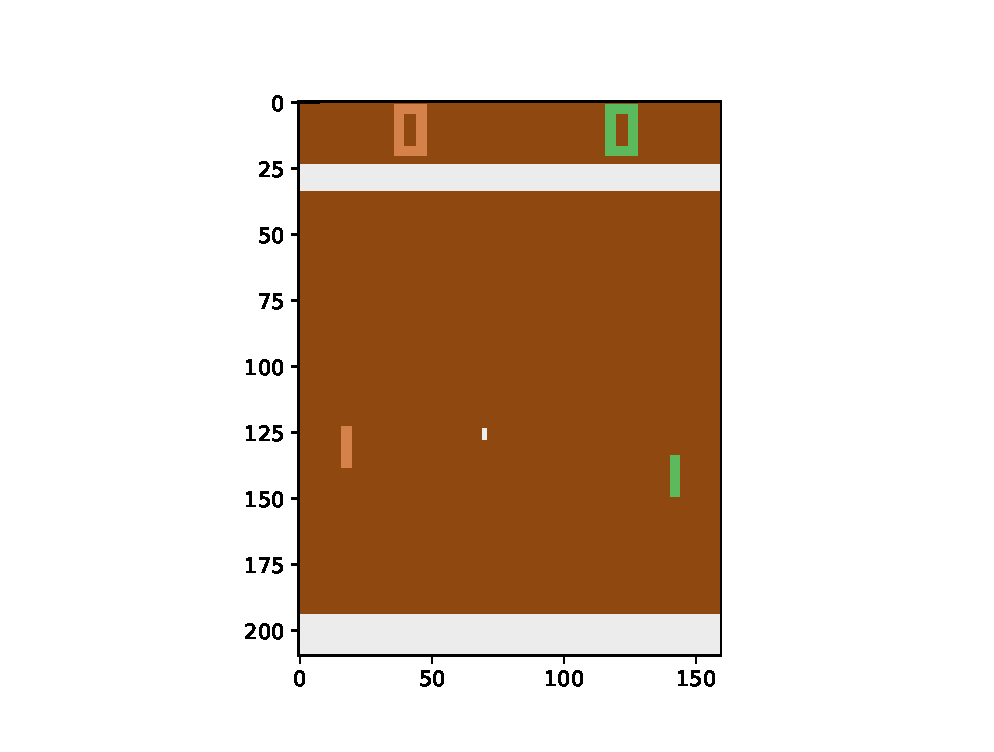
\includegraphics[width=\textwidth]{images/pong_example.eps}
\caption{Original Observation}
\end{subfigure}
\begin{subfigure}{0.45\textwidth}
\centering
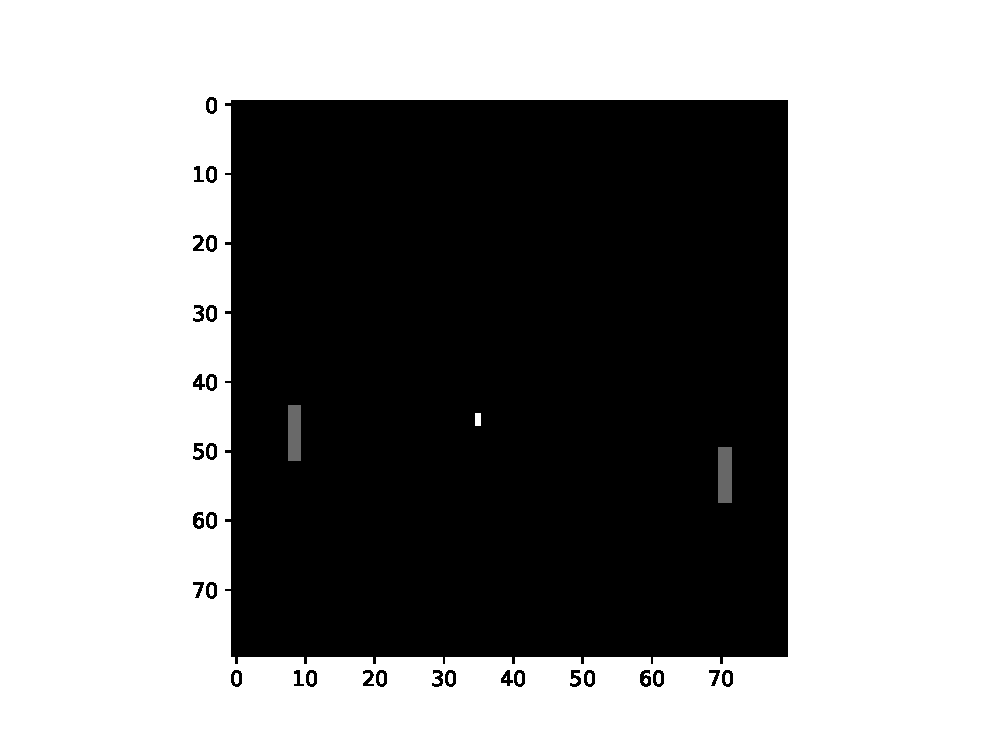
\includegraphics[width=\textwidth]{images/pong_preprocessed.eps}
\caption{Preprocessed Observation}
\end{subfigure}
\caption{Visualization of our preprocessing step}
\label{fig:preprocess}
\end{figure}


\subsection{Reward Clipping}

Different environments in the Atari gym have different reward structures, which means that training on the different games would mean that we need different hyper parameters and learning rates . To reduce this effect, we clip all non-zero rewards to either $1$, or $-1$. Of course, this will have a negative effect on the agent, since it cannot differentiate between small and big rewards. However, this does not have an effect in most games \cite{mnih2015human}.


\subsection{Replay Memory}
%Om patronen te voorkomen \cite{mnih2013playing}
Since we are playing the game in real time in the Atari environment, there will be a high correlation between successive game-states. Which might lead the algorithm to get stuck in a negative feedback loop. Consider the scenario in which moving to the right in the beginning of the game gives an immediate positive reward, but makes the player get stuck in some local maxima.

In order to mitigate this effect, we use experience replay \cite{mnih2013playing}. We let the network gather some experience, before we start training the network; we let the network play the game, and we store the current game state, the taken action, the resulting reward and the resulting game state and whether it was a final state to a list of experiences. After the network has gained enough experience, we start training the network. Training is done by uniformly sampling a experiences from the experience list which form our mini-batch. More details on training will be provided in chapter \ref{chapter:training}.

\subsection{Training details} \label{chapter:training}
%model initializatie + parameters etc. (qua hidden layers e.d.)
%Huber loss vs. MSE

The model is trained by utilizing the techniques mentioned before. The network will be trained to approximate the $Q^*$ function. Using the mean square error loss function:

\[
	L = \left(r + \gamma \max_{a'}( Q(\theta_i, s',a')) - Q(\theta_i, s, a)\right)^2
\]

in which $\theta_i$ are the current weights, $s'$ is the state that is obtained after performing $a$ on the state $s$, $r$ is the reward obtained by performing action $a$ on state $s$.

\subsection{Double DQN} \label{sec:doubleDQN}

Because the standard version of deep Q-learning uses the same $Q$ function to estimate the future reward and predict the current reward, there might arise feedback loops while training. To prevent this from happening, we can use two deep Q-networks called Double DQN \cite{van2016deep}. One network is used to predict the future reward and the action, and one is used to approximate the value that the network should predict. The adaptation of the loss function looks as follows

\[
	L = \left(r + \gamma \max_{a'}( Q(\bar\theta_i, s',a')) - Q(\theta_i, s, a)\right)^2
\]

in this function $\bar{\theta_i}
$ denotes the fact that the weights of this network are constant while training a single batch. 
We then synchronize model $\theta$ with $\bar\theta$ after a set number of frames. This leads to an increased stability in learning \cite{van2016deep}. Syncing is done by smoothing the difference between the weights of bother networks. One way how this is achieved is that the new weights are the average of the weights of the networks.


\subsubsection{Training}
Start the training by initializing the necessary things: initialize the weights of the network, initialize the experience list, initialize the Atari environment and set the current screen to be all zeros. After that, we can start training the network. 

Then we loop for some number of entire games over the entire next phase of the training. We use the network to decide the actions taken in the game. If a game is finished, we simply reset the environment and continue training, we also have to reinitialize the current game state. Every time an action is taken, we collect the current state, the action, the reward, and the next state and store these in the experience list. After we have gathered sufficient experience, we start training on this experience. This is done by sampling random experiences from the list, and using the values from the experience to calculate the loss, and do backpropagation with this loss, to estimate how we have to update the network. 





% is it useful to make some pseudocode
%\begin{algorithm}
%	\caption{My algorithm}\label{euclid}
%	\begin{algorithmic}
%\STATE f
%\end{algorithmic}
%\end{algorithm}
%




\section{Results}
In this section we will go over our results for CartPole and Pong. We will first give a quick explanation of the game followed by the results.


\begin{figure}[H]
\centering
\begin{subfigure}{0.45\textwidth}
\centering
\includegraphics[width=\textwidth]{images/cartpole.PNG}
\caption{CartPole Environment}
\label{fig:cartpole}
\end{subfigure}
\begin{subfigure}{0.45\textwidth}
\centering
\includegraphics[width=0.5\textwidth]{images/pong.png}
\caption{Pong Environment}
\label{fig:pong}
\end{subfigure}
\caption{Examples of Environments}
\end{figure}

\subsection{CartPole}
As a proof of concept we first tried to solve CartPole (env CartPole-v0), since this is the easiest environment to train on. In CartPole (figure \ref{fig:cartpole}) you control a cart. On top of this cart, there is a pole. The objective of this game is to balance the pole on the cart by moving the cart left or right. CartPole is considered `solved' when the average reward is greater than or equal to 195.0 over 100 consecutive trials.

The results of our algorithm may found in figure \ref{fig:cartpole_results}. What we can observe from these results is that the environment has a somewhat exponential learning curve until the ceiling has been reached (a score of 200). The algorithm fairly quickly learned what it should do. What we can observe from this result is that it seems that the agent was probably stuck in a local maxima at around 50 and 80 games. It probably tried to explore different options since the total reward drops. It took roughly 200 games to be good at the game. And after roughly 500 games, we solved CartPole by satisfying the win-condition.

\begin{figure}[H]
\centering
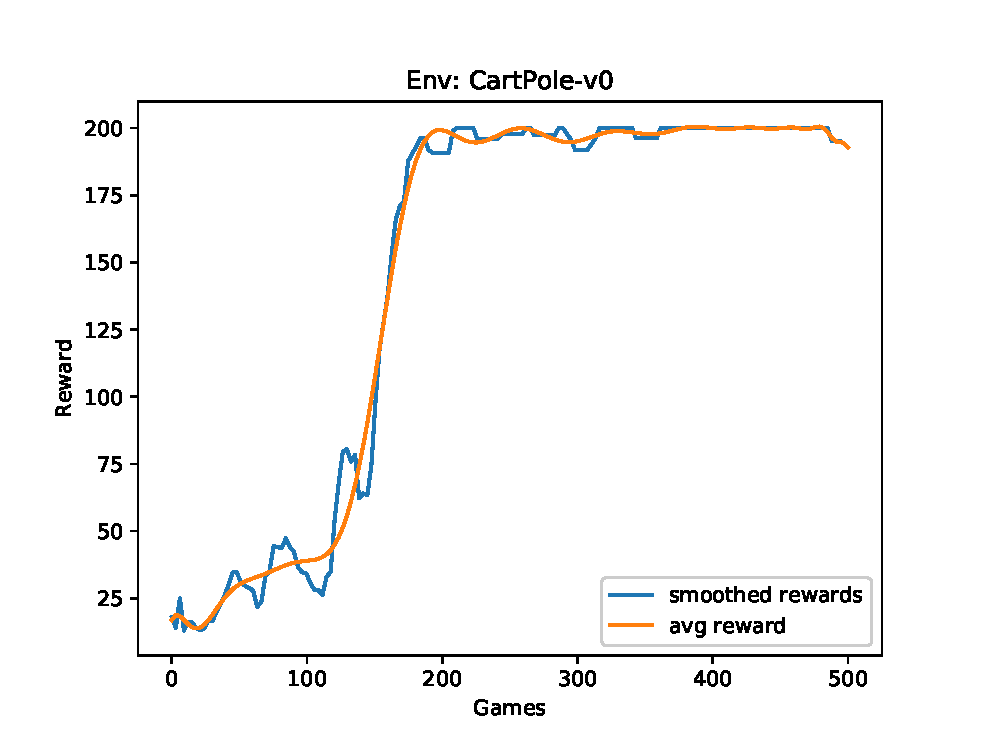
\includegraphics[width=0.5\textwidth]{images/cartpole_results.eps}
\caption{The result of the CartPole-v0 environment. The reward as a function of games.}
\label{fig:cartpole_results}
\end{figure}

\subsection{Pong}
The true test of our algorithm was Pong (env Pong-v0). In pong (figure \ref{fig:pong}), there are two players, on the left the AI and on the right the Player. The player can move their paddle up and down. The objective of the game is to get the ball behind the opponent and score a point. The player that first gets 21 games, has won the game.

Putting this into the context of our environment: scoring a point gives a reward of 1, losing gives a reward of -1. The game is over if a player has a score of 21. The total reward is the sum of all rewards, e.g. if the agent got a total reward of -21, he lost all games; if the player receives a total reward of 1, this means that he won 21 points and lost 20 times.

In figure \ref{fig:pong_results}, we see the results for game of Pong. The first thing that may be noticed when comparing this figure to figure \ref{fig:cartpole_results}, is that (effective) learning start much later: it took some 6000 games, before the agent finally started to learn. After some 9000 games, the reward becomes exponential. Using the win-condition that you win the game (e.g. a total reward of 1) for at least 100 subsequent games, then we did not solve Pong. However, since the learning is semi-exponential, assuming it is proportional to the total reward, we have confidence that when given more time, the agent would have beaten the opponent more often.

Another thing that we may observe is that the smoothed rewards still have a high variance. This is due to the instability of learning. Where weight-updates are too large, such that the weights `overshoot', e.g. over- or undervalue an action. This may be an indication that the learning rate was too high.
\begin{figure}[H]
\centering
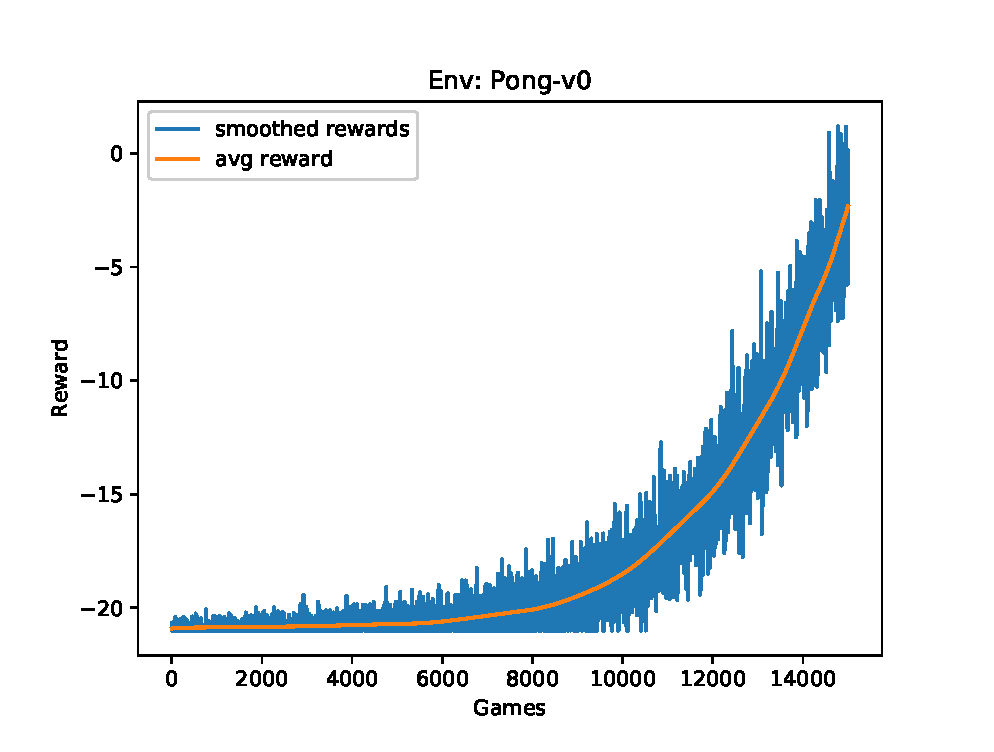
\includegraphics[width=0.5\textwidth]{images/pong_results.eps}
\caption{The result of the Pong-v0 environment. The reward as a function of games.}
\label{fig:pong_results}
\end{figure}

\section{Conclusion}
Although we were not able to train a network that fully beats any game apart from the easier CartPole, we can say with confidence that, given more time, the algorithm would eventually beat the criteria of beating Pong. We therefore show that the Google Deepmind paper \cite{mnih2013playing}, provides a good baseline for comparing algorithms for future reinforcement learning tasks. Since it is possible to train a network and achieve similar results as were reported in the paper.

\section{Discussion and Future Work}
%Complexer dan we dachten + link naar PNN
Although we have implemented the standard deep Q network, there are many different network structures that each have their own advantage and disadvantages. One particularly interesting network architecture is the Progressive Neural Network, this structures is specifically strong when learning different, but similar, games with the same network. Since knowledge learnt from previous games may help in learning new games.

Although we can train our network to act in the different games with relative ease, we have to start over from scratch each time we train the network, so extending our implementation to a Progressive Neural Network would be the next step in achieving generalized Reinforcement Learning.

The stability issues observed in the training of Pong (figure \ref{fig:pong_results}), may not be due to the learning rate or other parameters, but due to the nature of the model \cite{van2016deep}. A solution to this problem is to have two networks, one for network updating and one for smoothing the difference in weights when syncing as discussed in section \ref{sec:doubleDQN}.

In this paper, we had to scale down some parameters used in \cite{mnih2015human}, due to computation limitations. One of the parameters we scaled down is the capacity of the replay memory, where we used 1/40th of the capacity.


\bibliography{bibliography}
\bibliographystyle{plainnat}

\end{document}
